\pagenumbering{arabic}%start arabic pagination from 1 

\chapter{Platforma Vert.x}

Dnešním trendem internetu jsou real-time kolaborativní aplikace, které drasticky změnily potřeby programátorů, na jednotlivé nástroje. Programátor tak má možnost zvolit si z velké řádky nástrojů mezi než patří například Node.js, Akka či ruby EventMachine. Problémem těchto jinak časem a komunitou prověřených platforem může být fakt, že jsou úzce spjaté s konkretním programovacím jazykem či velmi náročná integrace do již stávájící aplikace.

Vert.x je projekt vycházející z Node.js, který jako první framework, pokořil v roce 2010 C10K\footnote{C10K problém řeší otázku: „Jak je možné obsloužit deset tisíc klientů za pomocí jednoho serveru, a to s co možná nejnižším zatížením serveru} problém. Platforma Vert.x má velice podobné API\footnote{Application Programming Interface} jako Node.js. Obě platformy poskytují kompletně asynchronní API. Jak již název napovídá Node.js je napsán v JavaScriptu, zatím co Vert.x je implementován v Javě. Vert.x ale nění pouhá reimplementace Node.js do jazyka Java. Platforma má svou vlastní unikátní filozofii, která je diametrálně odlišná od Node.js.

%Problém těchto jinak časem a komunitou ověřených platforem je fakt. Obě zmíněné platformy jsou napsány v dynamicky kompilovaném jazyku, což pro jádro stabilní aplikace přináší povinnost psát jak testy integrační, které testují funkčnost celého systému, tak i unit testy. 
%I když bude aplikace z větší části pokrytá testy, mohou se objevit problémy v podobě nečekaných pádů za běhu aplikace. To může být způsobeno například voláním neexistující metody či přiřazení proměnné do jiného typu než je ona sama. Toto bylo jedním z důvodů pro implementaci nového řešení v jazyce Java. Tento jazyk přináší platformě velkou stabilitu, rozšiřitelnost a zázemí v podobě tisícovek stabilních knihoven. Vert.x může být použit jako plnohodnotné řešení pro celou aplikaci nebo nasazen jako dílčí část architektury jiného řešení.

\section{Historie}

Začátek vývoje projektu Vert.x je datován do roku 2011. Tedy rok poté co spatřil světlo světa framework Node.js a za pouhý rok si vydobyl své místo u komunity, která si jej velmi oblíbila. Pravděpodobně největší motivací pro vývoj nové platformy podobné Node.js byla právě oblíbenost Node.js. 

Hlavním autorem platformy byl a je Tim Fox, který v době začátku vývoje platformy pracoval ve společnosti VMWare. Tato společnost si vzápětí nárokovala všechny zásluhy Tima Foxe na Vert.x platformu. Právníci společnosti vydaly výzvu, ve které požadovali mimo jiné doménu, veškerý zdrojový kód a účet Tima Foxe na Githubu. Z toho důvodu Tim Fox odešel od společnosti v roce 2012. V témže roce projevila o platformu zájem firma RedHat, která nabídla Timovi pracovní místo, absolutně volnou ruku ve vývoji a vedení projektu\citep{whoControlVertx}. 

Po několika debatách jak s představiteli společnosti RedHat tak i komunitou došel Tim Fox k názoru, že nejlepší pro budoucí zdravý rozvoj platformy bude přesunutí celé platformy pod nadaci Eclipse Foundation, k čemuž došlo na konci roku 2013. V dnešní době se platforma těší velkému vývoji, který čítá desítky  pravidelných přispěvatelů mezi něž patří mimo Tima například také Norman Maurer, který patří mezi přední inženýry vyvíjející framework Netty.io, který zodpovídá za integraci Netty frameworku do Vert.x platformy. Na tomto místě by bylo vhodné uvést, že platforma Vert.x letos vyhrála prestižní cenu "Most Innovative Java Technology" v soutěži JAX Innovation awards\citep{JAX}.

\section{Architektura}

\begin{figure}
\begin{centering}
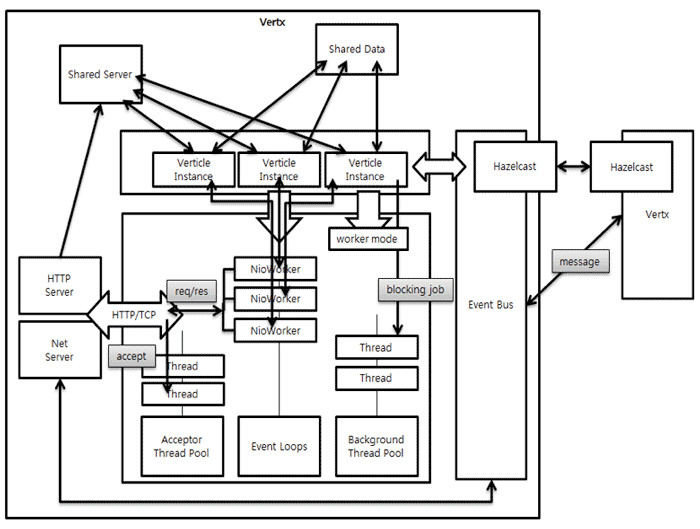
\includegraphics[width=1\textwidth]{obrazky/vertx-architecture-diagram}
\par\end{centering}
\caption{Architektura Vert.x \emph{Jaehong Kim} \label{fig:vertxArchitectureDiagram}}
\end{figure}

\subsection{Jádro}

Velikost samotného jádra aplikace nepřekračuje 10Mb kódu v jazyce java. V současné verzi je jádro platformy koherentní, dobře čitelné a poskytuje stabilní API. Lze jej následně rozšířit o novou funkčnost dokompilovaním balíčků, které lze naleznout v oficiálním repositáři. Pravděpodobnou inspirací byl již zmíněný Node.js respektive NPM\footnote{Node package manager} u kterého se takováto forma vývoje velice oblíbila. Od doby vzniku této platformy vzniklo nespočet rozšíření, které udělaly z Node.js silný násroj pro rychlý vývoj webových aplikací. 
Klíčové jsou aspekty jako událostmi řízené programování a neblokující asynchronní model. Událostmi řízené programování je podle Tomáše Pitnera\cite{javaProgramovani} základním principem tvorby aplikací s GUI(Graphical user interface). Netýká se však pouze GUI, je to obecnější pojem označující typ asynchronního programování, kdy je:
tok programu řízen událostmi;
události nastávají obvykle určitou uživatelskou akcí: klik či pohyb myši, stisk tlačítka
událostmi řízené aplikace musí být většinou programovány jako vícevláknové (i když spouštění vláken obvykle explicitně programovat nemusíme)
Asynchronní někdy také paralélní model je přímo závislý na způsobu implementace samotným programovacím jazykem. Základním pojmem je zde proces, který je vnímán jako jedna instance programu, který je plánován pro nezávislé vykonávání. Naproti tomu Vlákno\footnote{Označuje v informatice odlehčený proces, pomocí něhož se snižuje režie operačního systému při změně kontextu, které je nutné pro zajištění multitaskingu} je posloupnost po sobě jdoucích událostí.(vlákno). V dřívější době nebylo potřeba rozlišovat proces a vlákno, protože proces se dále v aplikaci nedělil. Základem Vert.x respektive Node.js je tedy vícevláknový model. V jedné aplikace tedy může běžet několik vláken. Vlákno je zde bráno jako základní plánovací jednotka pro běh na procesoru. 
Existují dva druhy asynchronního modelu (multitaskingu):
multiprocesorový: o běh, tvorbu a režii vláken se stará operační systém
multivláknový: o běh, tvorbu a režii vláken se stará aplikace a předává je operačnímu systému
Podle Lažanského\cite{vlaknaCvut} je sdílení paměti důsledkem nižší režie při přepínání (přepnutí vláken je výrazně rychlejší), obdobně i vytváření a rušení vlákna a samozřejmě i úspora paměti.
Jak již bylo zmíněno jádro Vert.x je implementováno v jazyce Java a zajímá nás tedy jak moc je dobrá implementace paralélního modelu. Zde se dostáváme k jedinému požadavku pro běh Vert.x instancí a to je přítomnost Java development Kitu ve verzi 1.7. Tato verze přinesla nespočet vylepšení, pro jejichž výpis zde není místo. Došlo také na přepsání či úpravy v několika zásadních třídách z balíčku java.util.concurrent\footnote{Knihovna pro práci s multitaskingem}.
\begin{description}
\item[ExecutorService]{z balíčku java.util.concurrent}
\item[CyclicBarrier\footnote{Synchronizační bariéra. Využitelná pro konstantní skupinu vláken, které mají přistupovat ke stejné proměnné. Třída zajištuje, že na sebe vlákna musí čekat při přístupu k proměnným. (Cyklická, protože jakmile se uvolní první vlákno jede to samé od znova)}]{z balíčku java.util.concurrent}
\item[CountDownLatch]{z balíčku java.util.concurrent}
\item[File]{z balíčku java.nio}
\item[Vylepšený ClassLoader]{lepší odolnost vůči deadlockům\footnote{ Odborný výraz pro situaci, kdy úspěšné dokončení první akce je podmíněno předchozím dokončením druhé akce, přičemž druhá akce může být dokončena až po dokončení první akce.}}
\end{description}
\emph{Více o java.concurrent\cite{javaChangelog}}

Ed Gardoh v roce 2011 ve svém jednoduchém testu\cite{serialTest} prověřil práci s paralelizací úkonů. Z jeho testů vyplývá, že Java 1.7 je až o 40\% rychlejší při práci s vlákny díky nové metodě Fork/Join\footnote{http://www.oracle.com/technetwork/articles/java/fork-join-422606.html}.

\subsubsection{základní API}\label{sub:coreAPI}

\begin{itemize}
\item{TCP/SSL server/klient}
\item{Websockets server/klient, SockJS}
\item{Event Bus / sdílená data}
\item{časovače}
\item{souborový systém}
\item{konfigurace}
\item{logování}
\end{itemize}

\subsubsection{Multi-reactor pattern}

Základ jádra je postaven na tzv. Multi-reactor pattern\cite{eventLoops}, který vychází z Reactor patternu\cite{reactorPattern}, ten lze charakterizovat několika body:

\begin{itemize}
\item{aplikace je řízena událostmi}
\item{na události se registrují handlery}
\item{vlákno zpracovává události a spouští registrované handlery}
\item{toto vlákno nesmí být blokováno\footnote{pokud dojde k zablkování hlavního vlákna dojde k zablokování celé aplikace např.\emph{Thread.sleep(), a další z java.util.concurrent }}}
\end{itemize}

Multi-reactor pattern\cite{eventLoops} se od Reactor patternu liší pouze tím, že může mít více hlavních vláken. Hlavní vlákno, kterému se okolo Vert.x komunity říká \emph{Event Loop}. V komunitách Nginx nebo Node.js se ovšem setkáme s pojmem \emph{Run Loop}. Tento návrhový vzor tedy převzala platforma z Node.js, kde se takovýto model velice oblíbil. Nevýhoda tohoto modelu je, že nikdy nesmí dojít k blokování hlavního vlákna a také fakt, že platforma Node.js poskytovala jenom jedno vlákno, které šlo škálovat na jednotlivé procesory. Jak je vidět z obrázku \vref{fig:instance} Vert.x platforma poskytuje více hlavních vláken, zpravidla však jedno hlavní vlákno na jeden procesor. Toho lze snadno docílit pomocí \emph{Runtime.getRuntime().availableProcessors()} na obrázku \vref{fig:instance4} lze vidět příklad čtyř hlavních vláken na čtyři dostupné procesory.
\vref
Příklady blokujících volání:
\begin{itemize}
\item{tradiční API (JDBC, externí systémy)}
\item{dlouhotrvající operace (generování apod.)}
\end{itemize}

\subsubsection{Hybridní model vláken}\label{sub:hybrid}

Platforma Vert.x přišla s inovací v oblasti hlavních vláken a to takovou, že k hlavním \emph{Event loops} přidala další sadu vláken \emph{Background thread pool}, které jsou vyčleněny z hlavní architektury a poskytující samostatnou kapitolu pro škálování aplikace. To lze ostatně vidět na obrázku \vref{fig:vertxArchitectureDiagram}. Díky tomu, lze psát specializované moduly nebo verticle tzv. \emph{workery} pro blokující volání či dlouhotrvající operace aniž by nějak omezovaly běh celé aplikace. Více o \emph{workerech} v \ref{sub:moduly}

\subsection{Vert.x instance}

Verticle běží v jedné Vert.x instanci \vref{fig:instance}. Každá Vert.x instance běží ve vlastním JVM instanci. V jedné Vert.x instanci může najednou běžet X Vertclů. Na jednom fyzickém stroji může běžet více Vert.x instancí případně v cluster módu i na více fyzických strojích.

\begin{figure}
\begin{centering}
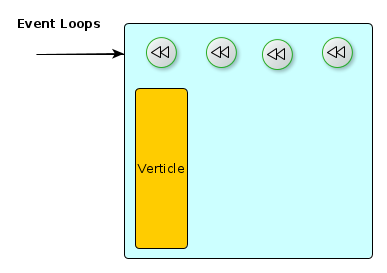
\includegraphics[scale=0.5]{obrazky/instance}
\par\end{centering}
\caption{Vert.x instance \label{fig:instance}}
\end{figure}

\begin{figure}
\begin{centering}
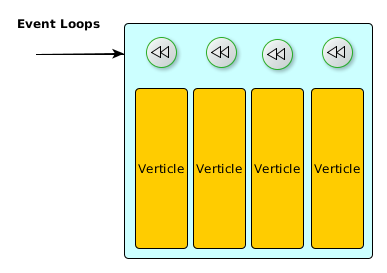
\includegraphics[scale=0.5]{obrazky/instance4}
\par\end{centering}
\caption{Vert.x instance \emph{vertx run HelloWord -instances 4} \label{fig:instance4}}
\end{figure}

\subsubsection{Verticle}

Základní jednotka vývoje a nasazení. Verticle může být skript nebo třída například v jazyce Java. Verticle lze spouštět samostatně\footnote{vertx run Verticle.js} v praxi se ovšem využívají pouze moduly, které obsahují zpravidla více Verticles popřípadě worker Verticles.

\begin{itemize}
\item nejmenší spustitelná jednotka
\item třída / skript
\item vykonává neblokující operace
\item konkurence - single-threaded\footnote{běží vždy pouze v jednom vlákně (odpadá synchronizace, zámky, ...), izolace (vlastní classloader)}
\item přístup ke Core API\ref{sub:coreAPI}, registrace handlerů, deploy dalších verticlů
\end{itemize}

Spuštění verticle programově
\begin{lstlisting}
JsonObject config = new JsonObject();
config.putString("foo", "wibble");
config.putBoolean("bar", false);
container.deployVerticle("foo.ChildVerticle", config);
\end{lstlisting}

Spuštění verticle z příkazové řádky
\begin{lstlisting}
vertx run foo.js -conf myconf.json
\end{lstlisting}

\subsubsection{Moduly} \label{sub:moduly}

Moduly poskytují větší míru zapouzdření a znovupoužitelnost funkcionality. V praxi se mohou moduly skládat z více modulů či verticlů a mohou být uloženy v centrálním repozitáři\footnote{http://modulereg.vertx.io/} nebo může být využit jakýkoliv jiný repozitář. Repozitáře v kterých hledá Vert.x při startu instance dostupné moduly lze definovat v hlavní konfiguraci Vert.x.
Každý modul musí mít svůj deskriptor ve formátu JSON\footnote{JSON (JavaScript Object Notation) je odlehčený formát pro výměnu dat. Je jednoduše čitelný i zapisovatelný člověkem a snadno analyzovatelný i generovatelný strojově.}, tento deskriptor musí být v kořenovém adresáři modulu a může vypadat například takto. \emph{toto je poze základní výčet parametrů všechny lze nalézt v dokumentaci Vert.x}

\begin{lstlisting}
{
  "main": "EchoServer.java",
  "worker": true,
  "includes": "io.vertx~some-module~1.1",
  "auto-redeploy": true
}
\end{lstlisting}

Typy modulů lze rozdělit do dvou základních skupin, které lze dál rozdělit podle typu určení modulu. 

\begin{description}
\item[spustitelné]{mají definovanou main třídu v deskriptoru, takovéto moduly je pak možné spustit jako samostatné jednotky pomocí parametru \emph{runmod nebo programově deployModule} }
\item[nespustitelné]{modul nemá specifikovanou main třídu a lze jej použít v jiném modulu použitím parametru \emph{includes}}
\end{description}

Jak bylo řečeno v \ref{sub:hybrid} Vert.x instance má dvě sady vláken. Parametrem \emph{worker} v deskriptoru modulu, lze říci Vert.x jádru aby spustil modul v \emph{background worker poolu}. Parametr \emph{auto-redeploy} mluví sám za sebe.

Spuštění modulu programově v jazyce Java
\begin{lstlisting}
container.deployModule("io.vertx~mod-mailer~2.0.0-beta1", JSONconfig);
\end{lstlisting}

Spuštění modulu z příkazové řádky
\begin{lstlisting}
vertx runmod com.mycompany~my-mod~1.0 -conf config.json
\end{lstlisting}

\subsubsection{Worker Verticle}

\subsection{Event Bus}

Nervový systém celého Vert.x. Cílem EventBusu je zpozdředkování komunikace mezi jednotlivými komponentami platformy. 
Nespornou výhodou je fakt, že lze takovouto komunikaci přemostit ke klientovi na straně webového prolížeče.

Základní typy komunikace:
\begin{itemize}
\item{Point to Point}
\item{Publish/Subscribe}
\end{itemize}

typy zpráv:
\begin{itemize}
\item{String}
\item{primitivní typy (int, long, short, float double, ..)}
\item{org.vertx.java.core.json.JsonObject}
\item{org.vertx.java.core.buffer.Buffer}
\end{itemize}

Toto jsou pouze základní typy zpráv, které Vert.x podporuje v základu. Není ale vůbec problém výčet stávájících typů rozšířit(doimplementovat). Například modul bson.vertx.eventbus\footnote{https://github.com/pmlopes/mod-bson-io} rozšíří aplikaci o možnost používat mnohem komplexnější typy zpráv. Mezi doporučené se ovšem řadí JSON, protože je jednoduše serializovatelný mezi jednotlivými programovacími jazyky.
\begin{itemize}
\item{java.util.UUID}
\item{java.util.List}
\item{java.util.Map}
\item{java.util.Date}
\item{java.util.regex.Pattern}
\item{java.sql.Timestamp}
\end{itemize}

\subsection{Hazelcast}

Jednou z nejdůležitějších architektonických součástí Vert.x je knihovna Hazelcast\footnote{okolo 2.6MB kódu v jazyce Java, In-Memory Data Grid (IMDG)}, Hlavní výhody In-memory data grid\cite{inMemoryDataGrid} lze podle Ki Sun Song sumarizovat:
\begin{itemize}
\item{Data jsou distribuovaná a uložená na více servrech }
\item{Datový model je většinou objektově orientovaný a ne-relační}
\item{Každý server pracuje v aktivním režimu}
\item{Dle potřeby lze přidávat a odebírat servery}
\end{itemize}

Hazelcast lze využít v několika rolích:
\begin{itemize}
\item{In-memory NoSQL\footnote{databázový koncept, ve kterém datové úložiště i zpracování dat používají jiné prostředky než tabulková schémata tradiční relační databáze}}
\item{Caching\footnote{specializovaný typ paměti pro krátkodobé ukládání}}
\item{Data grid}
\item{Messaging}
\item{Application Scaling}
\item{Clustering}
\end{itemize}

Hazelcast je tedy typ distribuovaného úložiště, které běží jako embedded a lze díky němu distribuovat celou aplikaci. Hazelcast API je využíváno přes API Vert.x. Když je Vert.x spuštěn, Hazelcast je spuštěn v embedded\footnote{Hazelcast server je spuštěn jádrem Vert.x} módu. 
Jako nejčastější příklad bývá uváděno ukládání uživatelské session\footnote{Session v protokolu HTTP dává webovému serveru možnost uložit si libovolné (většinou však ne příliš obsáhlé) informace o uživatelích, kteří k němu přistupují, a to o každém zvlášť. Protokol HTTP ze svého principu (a způsobu komunikace stylem požadavek - odpověď) postrádá kontext o jednotlivých klientech, a právě session ho webovým aplikacím dokáže dát.} Hazelcast tedy usnadní práci v situaci, kdy budeme potřebovat uložit uživatelskou session například pro eshop. Mohli bychom využít využit externí RDBMS\footnote{Databázový server, který spravuje databáze, komunikaci s klienty (lokálními nebo vzdálenými), vstupy a výstupy dat a jejich integritu.} díky, kterému by jsme dosáhli stejného výsledku. Hazelcast nám ovšem zaručí replikování mezi jednotlivými servery, fail-over S využitím embedded Hazelcast ovšem odpadá nezbytná režie a monitoring, nemluvě o serverových prostředcích.

Proto ty, kteří potřebují ukládat uživatelské session pro E-commercy či chat-servery toho mohou jednoduše dosáhnout skrz konfiguraci samotného Vert.x.


\section{Test}
Ed Gardoh v roce 2011 provedl test\cite{serialTest} pro porovnání paralelizace\footnote{Paralelizace procesů se skládá z rozložení jednoho velkého úkonu do několika menších úkolů, které mohou běžet paralelně.Výsledkem je provedení jednoho úkolu nebo procesu za pomocí více než jednoho procesoru nebo procesorů "Paralelní zpracování", nesmí být zaměňováno se souběžností.} v Javě 1.6 a 1.7.
Hlavní myšlenkou je aby testovací třída simulovala úkol, který jako první volá vzdálenou službu a čeká sekundu na výzvu k návratu(spánek) a pak simuluje nějaké zpracování s výsledkem, jako je formátování řetězce.
\vref{fig:serialtestI} je vidět synchronní běh serializační třídy v Javě 1.6. Z \vref{fig:serialCputestI} je pak vidět využití potenciálů jednotlivých procesorů.
Výsledek není žádné překvapení 50 úkolů s 1 sekundovým spánkem a spojováním řetězce trvalo něco málo přes 65 sekund. 
Cílem jeho testu mělo být porovnání paralelizování úkonů. Výsledky testu ukázaly zlepšení až o 75\%. Z obrázků 1-4 zřetelně plyne, že nová Java je, pro single-thread\footnote{jedno vláknový} model aplikace ta nejlepší volba.

Jetnotlivé testy prokázaly, že za takovým rapidním zrychlením stojí metody Fork/Join. Při vhodném škálování bylo zrychlení až o 75\%. Z testů ovšem vyplívá také fakt, že při neúměrném počtu hlavních vláken na počet procesorů to má negativní dopady. Jedním z dopadů je 100\% vytížení a jednotlivých jader. Při vhodném určení počtu vláken, je vidět rapidní urychlení asynchronní paralelizace. Node.js i Vert.x však poskytuji informace o celkovém počtu fyzických jader procesoru a ta je tedy snadné určení optimálního počtu vláken pro ideální výsledky.(Více na?asi vysvětlit)

\begin{figure}
\begin{centering}
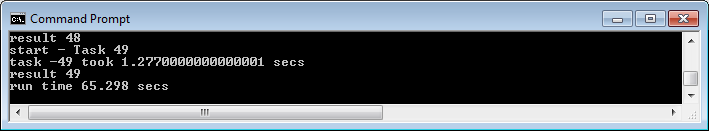
\includegraphics[width=1\textwidth]{obrazky/serial_test_r1}
\par\end{centering}
\caption{První test běhu serializační třídy \label{fig:serialtestI}}
\end{figure}

\begin{figure}
\begin{centering}
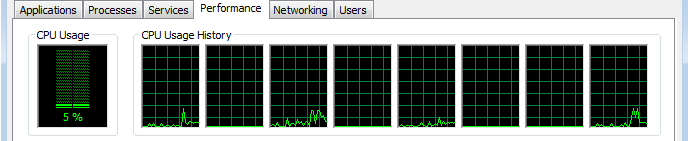
\includegraphics[width=1\textwidth]{obrazky/serial_cpu_1}
\par\end{centering}
\caption{Využití jednotlivých procesorů při běhu \label{fig:serialCputestI}}
\end{figure}

\begin{figure}
\begin{centering}
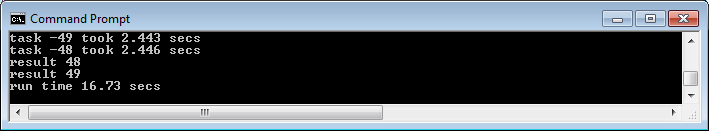
\includegraphics[width=1\textwidth]{obrazky/executor_test_r1}
\par\end{centering}
\caption{První test běhu serializační třídy \label{fig:executorTestI}}

\end{figure}

\begin{figure}
\begin{centering}
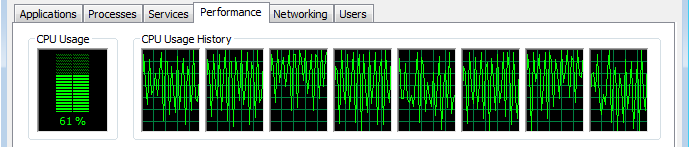
\includegraphics[width=1\textwidth]{obrazky/executor_cpu_1}
\par\end{centering}
\caption{První test běhu serializační třídy \label{fig:executorCpuTestI}}

\end{figure}
